\documentclass[11pt, a4paper]{article}
\usepackage[utf8]{inputenc}
\usepackage{amsmath, amssymb}
\usepackage{graphicx}
\usepackage{hyperref}
\usepackage{geometry}
\geometry{margin=1in}

\title{EE 325 Digital Signal Processing \\ Assignment 9: Discrete Fourier Transform (DFT) and Properties}
\author{PERERA J.D.T. \\ E/21/291}
\date{\today}

\begin{document}
\maketitle

\section{1. DFT Computation by Hand}
Compute the 4-point DFT of $x[n] = \{1, 2, 0, 0\}$ for $n = 0, 1, 2, 3$.

\subsection{(a) Using the DFT formula}
The $N$-point DFT is given by:
$$ X[k] = \sum_{n=0}^{N-1} x[n] e^{-j \frac{2\pi}{N} kn } $$
For $N = 4$ and given $x[n]$, only $n=0$ and $n=1$ have non-zero terms:
$$ X[k] = x[0] e^{0} + x[1] e^{-j \frac{2\pi}{4} k(1)} = 1 + 2e^{-j \frac{\pi}{2} k} = 1 + 2(-j)^k $$

Evaluating for $k = 0, 1, 2, 3$:
\begin{itemize}
    \item $k = 0: X[0] = 1 + 2(-j)^0 = 1 + 2(1) = 3$
    \item $k = 1: X[1] = 1 + 2(-j)^1 = 1 - 2j$
    \item $k = 2: X[2] = 1 + 2(-j)^2 = 1 + 2(-1) = -1$
    \item $k = 3: X[3] = 1 + 2(-j)^3 = 1 + 2(j) = 1 + 2j$
\end{itemize}

\subsection{(b) Results in rectangular form}
\begin{itemize}
    \item $X[0] = 3 + j0$
    \item $X[1] = 1 - j2$
    \item $X[2] = -1 + j0$
    \item $X[3] = 1 + j2$
\end{itemize}
\textbf{Note:} Since $x[n]$ is real-valued, $X[k]$ exhibits conjugate symmetry $X[k] = X^*[N-k]$. Here, $X[1] = X^*[3] = 1 - 2j$.

\section{2. Parseval's Theorem}
Using $X[k]$ from Q1 to verify Parseval's theorem.

\subsection{(a) Time-domain energy $E_x$}
$$ E_x = \sum_{n=0}^{3} |x[n]|^2 = |1|^2 + |2|^2 + |0|^2 + |0|^2 = 1 + 4 = 5 $$

\subsection{(b) Frequency-domain energy $E_X$}
$$ E_X = \frac{1}{N} \sum_{k=0}^{3} |X[k]|^2 $$
First, compute the squared magnitudes $|X[k]|^2$:
\begin{itemize}
    \item $|X[0]|^2 = 3^2 = 9$
    \item $|X[1]|^2 = 1^2 + (-2)^2 = 1 + 4 = 5$
    \item $|X[2]|^2 = (-1)^2 = 1$
    \item $|X[3]|^2 = 1^2 + 2^2 = 1 + 4 = 5$
\end{itemize}

$$ E_X = \frac{1}{4} (9 + 5 + 1 + 5) = \frac{1}{4} (20) = 5 $$

\subsection{(c) Verification}
Since $E_x = 5$ and $E_X = 5$, Parseval's theorem is verified:
$$ \sum_{n=0}^{N-1} |x[n]|^2 = \frac{1}{N} \sum_{k=0}^{N-1} |X[k]|^2 $$

\section{3. Python – Convolution via DFT}

\subsection{(a) Linear Convolution}
Given $x[n] = [1, 2, 3]$ and $h[n] = [1, 1, 1]$. \\
The linear convolution length is $L_x + L_h - 1 = 3 + 3 - 1 = 5$. \\
Using `numpy.convolve`, the linear convolution $y_{lin}[n]$ is derived as:
$$ y_{lin}[n] = [1, 3, 6, 5, 3] $$

\subsection{(b) 3-point DFT Circular Convolution}
Computing the 3-point DFTs of $x[n]$ and $h[n]$, multiplying them, and taking the 3-point IDFT gives the 3-point circular convolution $y_{circ3}[n]$.
$$ y_{circ3}[n] = [6, 6, 6] $$
\textbf{Comparison:} $y_{circ3}[n]$ does not match $y_{lin}[n]$. The values are corrupted due to \textit{time-domain aliasing} (circular wrap-around) because the DFT length $N=3$ is less than the required linear convolution length $L = 5$. The overlapping tails from index $n \ge 3$ of the linear convolution wrap around and add to the beginning:
$$ y_{circ3}[0] = y_{lin}[0] + y_{lin}[3] = 1 + 5 = 6 $$
$$ y_{circ3}[1] = y_{lin}[1] + y_{lin}[4] = 3 + 3 = 6 $$
$$ y_{circ3}[2] = y_{lin}[2] = 6 $$

\subsection{(c) 5-point Zero-Padded DFT Convolution}
By zero-padding $x[n]$ and $h[n]$ to a length of $N = 5 \ge L_x + L_h - 1$, the 5-point circular convolution yields:
$$ y_{circ5}[n] = [1, 3, 6, 5, 3] $$
This result matches exactly with the linear convolution $y_{lin}[n]$.

\textbf{Explanation of Circular vs. Linear Convolution Using DFT:}
This demonstrates that multiplication in the frequency domain (DFT domain) corresponds to \textit{circular convolution} in the time domain, not linear convolution. 
To obtain the linear convolution of two sequences using the DFT (which represents circular convolution), the sequences must be explicitly zero-padded to a length $N \ge L_x + L_h - 1$. This padding provides enough "empty space" to prevent the time-domain alias wrap-around, effectively making the discrete periodic convolution identical to the linear convolution over a single period.

\begin{figure}[h]
    \centering
    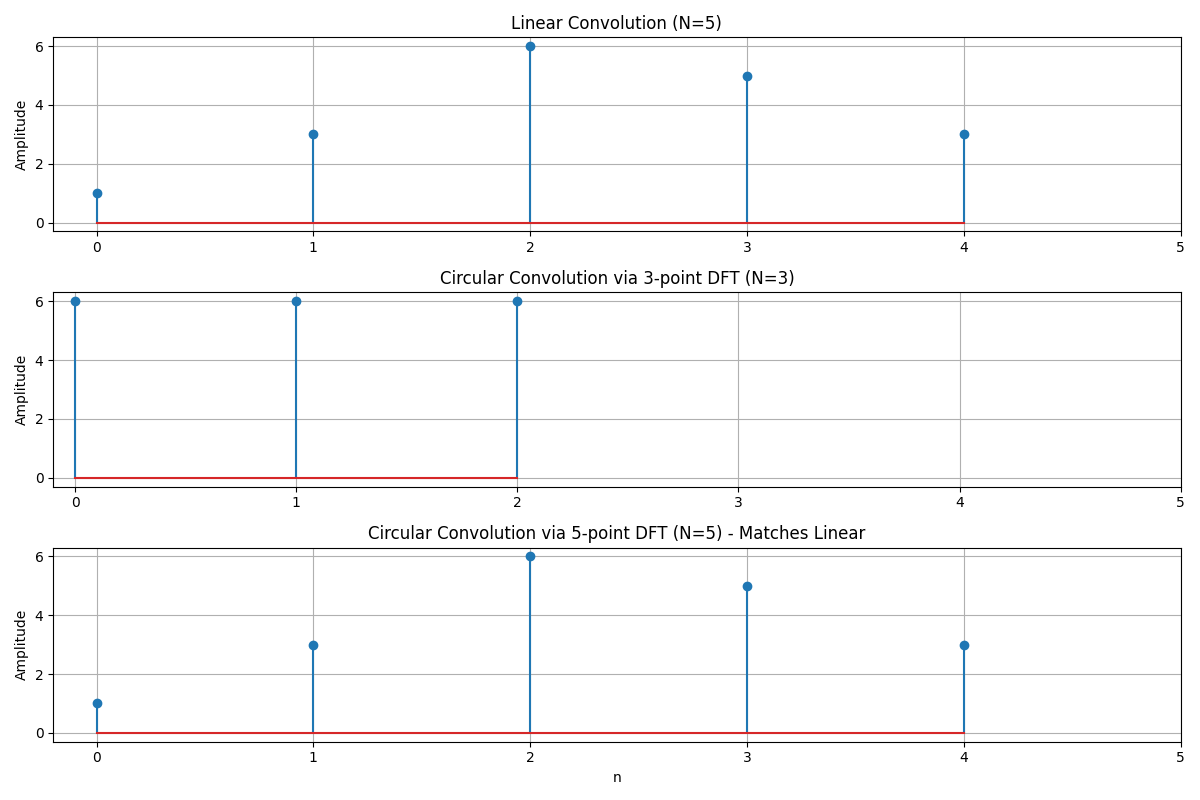
\includegraphics[width=0.8\textwidth]{plots/convolution_comparison.png}
    \caption{Convolution Comparison: Linear vs Circular}
    \label{fig:conv_comp}
\end{figure}

\end{document}
